\documentclass[crop,border={2pt 2pt 2pt 2pt},tikz]{standalone}
\usepackage{braket}
\usepackage{bbold}
\usepackage{bm}


\usetikzlibrary{backgrounds,decorations.markings}
\tikzset{>=latex}
\tikzset{->-/.style={decoration={
  markings,
  mark=at position .5 with {\arrow{>}}},postaction={decorate}}}
\begin{document}
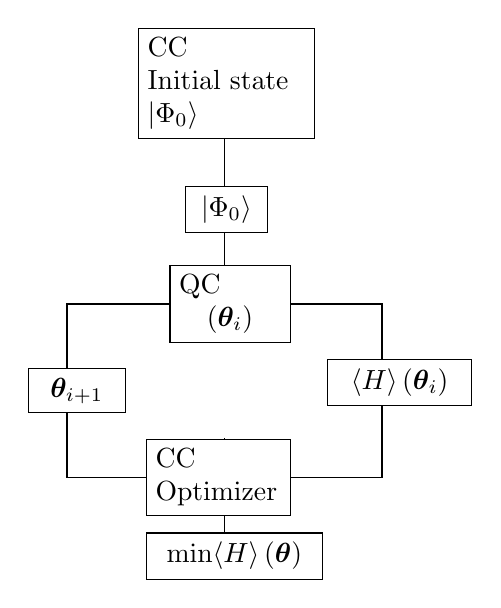
\begin{tikzpicture}
    \draw[black] (3.5,3) -- (3.5,0.2) -- (5.5,0.2) -- (5.5, -2) -- (1.5,-2) -- (1.5,0.2) -- (3, 0.2);
    \draw[black] (3.5, -1.5) -- (3.5, -3);
    \node[draw,fill=white, anchor=west, text width=2cm] at (2.4,3) {CC \\ 
    Initial state $\ket{\Phi_0}$ };
    \node[draw,fill=white,anchor=west,text width=0.8cm, align=center] at (3,1.4) {$\ket{\Phi_0}$};
    \node[draw,fill=white,anchor=west, text width=1.3cm] at (2.8,0.2) {QC \\
    $\ \ \  (\bm \theta_i)$};
    \node[draw,fill=white,anchor=west,text width=1.6cm, align=center] at (4.8,-0.8) {$\braket{H}(\bm \theta_i)$};
    \node[draw,fill=white,anchor=west,text width=1.6cm] at (2.5,-2) {CC \\ 
    Optimizer};
    
    \node[draw,fill=white,anchor=west,text width=1cm, align=center] at (1,-0.9) {$\bm \theta_{i+1}$};

    \node[draw,fill=white,anchor=west,text width=2cm, align=center] at (2.5,-3) {min$\braket{H}(\bm \theta)$};





    % \node[anchor=west, text width=1.4cm, align=center] at (-1.7,-1.5) {Original signal. $k$ bits.};
    % \node[fill=white,anchor=west,text width=2cm, align=center] at (0.4,-1.5) {Adds redundancy. $k\rightarrow n$ bits.};
    % \node[fill=white,anchor=west,text width=2cm, align=center] at (2.5,-1.5) {May randomly flip bits.};
    % \node[fill=white,anchor=west,text width=2cm, align=center] at (4.5,-1.5) {Restores the information.\\ $n\rightarrow k$ bits.};
    % \node[anchor=west, text width=1.4cm,align=center] at (7,-1.5) {Restored signal. $k$ bits.};
\end{tikzpicture}
\end{document}
 
